% Options for packages loaded elsewhere
\PassOptionsToPackage{unicode}{hyperref}
\PassOptionsToPackage{hyphens}{url}
\documentclass[
]{article}
\usepackage{xcolor}
\usepackage{amsmath,amssymb}
\setcounter{secnumdepth}{-\maxdimen} % remove section numbering
\usepackage{iftex}
\ifPDFTeX
  \usepackage[T1]{fontenc}
  \usepackage[utf8]{inputenc}
  \usepackage{textcomp} % provide euro and other symbols
\else % if luatex or xetex
  \usepackage{unicode-math} % this also loads fontspec
  \defaultfontfeatures{Scale=MatchLowercase}
  \defaultfontfeatures[\rmfamily]{Ligatures=TeX,Scale=1}
\fi
\usepackage{lmodern}
\ifPDFTeX\else
  % xetex/luatex font selection
\fi
% Use upquote if available, for straight quotes in verbatim environments
\IfFileExists{upquote.sty}{\usepackage{upquote}}{}
\IfFileExists{microtype.sty}{% use microtype if available
  \usepackage[]{microtype}
  \UseMicrotypeSet[protrusion]{basicmath} % disable protrusion for tt fonts
}{}
\makeatletter
\@ifundefined{KOMAClassName}{% if non-KOMA class
  \IfFileExists{parskip.sty}{%
    \usepackage{parskip}
  }{% else
    \setlength{\parindent}{0pt}
    \setlength{\parskip}{6pt plus 2pt minus 1pt}}
}{% if KOMA class
  \KOMAoptions{parskip=half}}
\makeatother
\usepackage{longtable,booktabs,array}
\usepackage{caption}
\captionsetup[table]{skip=6pt}
\newcounter{none} % for unnumbered tables
\usepackage{calc} % for calculating minipage widths
% Correct order of tables after \paragraph or \subparagraph
\usepackage{etoolbox}
\makeatletter
\patchcmd\longtable{\par}{\if@noskipsec\mbox{}\fi\par}{}{}
\makeatother
\usepackage{graphicx}
\makeatletter
\newsavebox\pandoc@box
\newcommand*\pandocbounded[1]{% scales image to fit in text height/width
  \sbox\pandoc@box{#1}%
  \Gscale@div\@tempa{\textheight}{\dimexpr\ht\pandoc@box+\dp\pandoc@box\relax}%
  \Gscale@div\@tempb{\linewidth}{\wd\pandoc@box}%
  \ifdim\@tempb\p@<\@tempa\p@\let\@tempa\@tempb\fi% select the smaller of both
  \ifdim\@tempa\p@<\p@\scalebox{\@tempa}{\usebox\pandoc@box}%
  \else\usebox{\pandoc@box}%
  \fi%
}
% Set default figure placement to htbp
\def\fps@figure{htbp}
\makeatother
\setlength{\emergencystretch}{3em} % prevent overfull lines
\providecommand{\tightlist}{%
  \setlength{\itemsep}{0pt}\setlength{\parskip}{0pt}}
\usepackage{bookmark}
\IfFileExists{xurl.sty}{\usepackage{xurl}}{} % add URL line breaks if available
\urlstyle{same}
% fallback for those not using the hyperref driver hyperxmp:
\makeatletter
\@ifundefined{xmpquote}{\newcommand{\xmpquote}[1]{#1}}{}
\makeatother
\hypersetup{
  hidelinks,
  pdfcreator={LaTeX via pandoc}}

\author{}
\date{}

\begin{document}

\section{Receiver Feedback and Timely Source-Update Availability in a
Cooperative-Perception
Simulation}\label{receiver-feedback-and-timely-source-update-availability-in-a-cooperative-perception-simulation}

\textbf{Dipesh Gurung}ᵃ, \textbf{Binod Bhattarai}ᵇ*,
\textbf{Prof.~Dr.~R. N. Thakur}ᵃ

ᵃ \emph{Research Department, Lord Buddha Education Foundation (LBEF
College), Opposite to Maitidevi Temple, Kathmandu 44600, Nepal}\\
ᵇ \emph{Department of Computer Science and Engineering, School of
Sciences, Noida International University (NIU), Greater Noida, Uttar
Pradesh 203201, India}

* Corresponding author.\\
\emph{Email addresses:} dipesh.gurung@lbef.edu.np (D. Gurung),
binoth25@gmail.com (B. Bhattarai), rn.thakur@lbef.edu.np (R. N.
Thakur)\\
\emph{ORCID:} 0009-0009-0335-2267 (D. Gurung), 0009-0006-6691-5264 (B.
Bhattarai), 0000-0003-3911-4358 (R. N. Thakur)

\subsection{Highlights}\label{highlights}

\begin{itemize}
\tightlist
\item
  Evaluates V2V cooperative perception under 802.11p radio and receiver
  queueing.
\item
  Receiver offered load reaches 0.571 at 3 ms and exceeds 1.0 at 6 ms
  service.
\item
  In tested paired runs, fixed 10 Hz transmission had higher success
  than feedback.
\item
  93.38\% of joint-policy rate decreases were labeled backlog-only.
\end{itemize}

\subsection{Abstract}\label{abstract}

This paper compares sender policies for timely authenticated
source-update availability in a controlled cooperative-perception
simulation. The model combines ns-3.46.1 802.11p broadcast with one
finite first-come, first-served (FCFS) verification worker per receiver.
Verification is represented by deterministic synthetic service-time
budgets; signatures are assumed valid. We evaluated distinct exploratory
experiment families: a 180-run factorial campaign (three seeds per
cell), a stress sweep with 65 trace-audited runs out of 75, a 35-run
threshold ablation, and an 80-run paired comparison at one operating
point. In the paired comparison (48 sources, intersection geometry, 3 ms
service, 20 paired seeds), mean same-opportunity success was 94.75\% for
fixed 10 Hz transmission, 81.98\% for the project radio-only controller,
15.84\% for uncalibrated joint feedback, and 55.91\% for calibrated
feedback. Calibrated feedback exceeded uncalibrated joint feedback by
40.07 percentage points (paired 95\% t interval half-width 4.18 points;
Cohen's dz = 4.49), while remaining 38.83 points below fixed
transmission and 26.07 points below radio-only control. These results
describe this model and operating point; the paired study is exploratory
and includes no DCC comparator. A separate fixed-policy arrival analysis
estimated mean offered load of 0.571 at 3 ms and 1.143 at 6 ms. Offered
load is not measured processor utilization. The model uses synthetic
demand, mobility, payloads, service times, and propagation, and has no
object-level perception or safety outcome. The findings therefore do not
establish hardware performance, deployment efficacy, or vehicle-safety
benefit.

\textbf{Keywords:} Cooperative perception; Receiver queue; Radio
contention; Feedback control; Discrete-event simulation; Information
freshness

\subsection{1. Introduction}\label{introduction}

Cooperative-perception systems exchange information among vehicles or
infrastructure nodes to support a shared representation of nearby
conditions. Message-generation and congestion-control studies have
considered how transmission frequency, message content, and access-layer
behavior affect channel use {[}1, 2{]}. Standards also define
cooperative-perception message services and access-layer
congestion-control mechanisms {[}3, 4{]}. Separately, vehicular security
and communication-computation research have modeled processing delay,
multi-agent coordination, and information freshness {[}5--8{]}. These
lines of work provide context for studying communication and receiver
processing in one simulated pipeline.

This study examines a limited comparison: under common periodic
source-update demand in the implemented simulator, how do fixed
transmission, radio-only rate control, receiver-load feedback, and a
project DCC mapping compare on whether each eligible opportunity's own
update becomes authenticated and fusion-ready before a configured
deadline? The simulation represents verification with an input service
duration. It does not execute cryptography or validate certificates. Its
outcomes concern update timing, not object detection, tracking, driving
decisions, or safety.

The principal comparison is a 20-seed paired experiment at one setting:
48 sources, synthetic intersection geometry, and a 3 ms deterministic
verification service time. Other campaigns characterize different
questions and are reported separately. All analyses are treated as
exploratory because the project folder does not establish a dated
pre-analysis freeze.

\subsubsection{1.1. Contributions and
scope}\label{contributions-and-scope}

This paper contributes a comparative simulation characterization of
sender policies under the stated model, together with an audited
operational definition of same-opportunity timely success and separate
deadline-freshness coverage. It reports an exploratory paired
comparison, a separately audited stress sweep and threshold ablation,
and a receiver-level offered-load calculation. It does not claim a new
controller, queueing theory, freshness metric, standards implementation,
hardware benchmark, or safety result. The conclusions are conditional on
the specified demand, radio, mobility, queue, service, and policy
settings.

\subsection{2. Related work}\label{related-work}

Cooperative-perception research has examined how message content and
transmission frequency affect channel use and the information available
to receiving vehicles. Thandavarayan et al.~evaluated congestion control
in cooperative-perception scenarios, while a separate paper by the same
authors studied generation and organization of cooperative-perception
messages {[}1, 2{]}. Muhammad et al.~analyzed security-related delay
across sender, radio, and receiver stages in broadcast V2V communication
{[}5{]}. These works motivate considering communication and processing
in a shared timing path, without implying that the present simulator
reproduces their models.

For freshness and scheduling, Wang et al.~studied age-constrained
scheduling for asynchronous updates in collaborative perception {[}6{]}.
Chen et al.~introduced Age of Computing metrics for communication and
computation cooperative networks with deadline models {[}7{]}. Recent
work by Tian et al.~introduced Sense2Com {[}8{]}, a multi-agent
reinforcement learning framework that coordinates sensing target
selection, V2V communication, and computation offloading for cooperative
perception. While Sense2Com addresses communication-computation
trade-offs by formulating sender-side sensing selection, transmission
scheduling, and computational offloading under reinforcement learning,
its stated model centers on transmission and offloading coordination
rather than receiver-side cryptographic signature-verification queues or
certificate backlog dynamics under broadcast reception. These studies
use different system models and outcomes from the same-opportunity
success measure defined here. Their existence also means that this paper
makes no novelty claim for combining queueing, feedback, or freshness
concepts.

ETSI specifications describe the Collective Perception Service and
access-layer decentralized congestion control {[}3, 4{]}. They are
standards context, not validation of this implementation. The
\texttt{dcc} policy is a limited project mapping; it is not a full
ITS-G5 facilities-layer implementation or a conformance claim.

This bounded literature inspection is not a systematic review.
Additional recent candidates, including Load-Aware Agent Selection via
delay prediction (Miyata et al., to appear) and a dynamic priority-based
batch verification scheme (DPBV, 2025), are deferred pending published
proceedings and full-text retrieval, respectively, and are recorded in
the project literature matrix; no detailed comparison is made here.

\subsubsection{Table 1. Selected literature
context}\label{table-1.-selected-literature-context}

{\def\LTcaptype{none} % do not increment counter
\begin{longtable}[]{@{}
  >{\raggedright\arraybackslash}p{(\linewidth - 6\tabcolsep) * \real{0.2500}}
  >{\raggedright\arraybackslash}p{(\linewidth - 6\tabcolsep) * \real{0.2500}}
  >{\raggedright\arraybackslash}p{(\linewidth - 6\tabcolsep) * \real{0.2500}}
  >{\raggedright\arraybackslash}p{(\linewidth - 6\tabcolsep) * \real{0.2500}}@{}}
\toprule\noalign{}
\begin{minipage}[b]{\linewidth}\raggedright
Work
\end{minipage} & \begin{minipage}[b]{\linewidth}\raggedright
Scope inspected
\end{minipage} & \begin{minipage}[b]{\linewidth}\raggedright
Relevance to this study
\end{minipage} & \begin{minipage}[b]{\linewidth}\raggedright
Evidence boundary
\end{minipage} \\
\midrule\noalign{}
\endhead
\bottomrule\noalign{}
\endlastfoot
Thandavarayan et al.~(2020) {[}1{]} & Cooperative-perception
congestion-control evaluation & Communication-control context & Distinct
from the message-generation paper {[}2{]} \\
Thandavarayan et al.~(2020) {[}2{]} & Cooperative-perception message
generation & Message-generation context & No claim that this simulation
implements those generation rules \\
Muhammad et al.~(2019) {[}5{]} & Security-related broadcast delay and
queueing analysis & Prior analytical treatment of communication and
processing delay & Does not supply the synthetic service-time settings
used here \\
Wang et al.~(2023) {[}6{]} & Age-constrained scheduling for asynchronous
collaborative-perception updates & Freshness and scheduling context &
Different system model and outcome definition \\
Chen et al.~(2025) {[}7{]} & Computation freshness and deadline models &
Computation-timeliness context & Not a vehicle broadcast or
signature-verification experiment \\
Tian et al.~(2026) {[}8{]} & Joint sensing, communication, and
computation coordination (Sense2Com) & Communication-computation
trade-off context & Stated focus is on sender-side sensing selection,
transmission scheduling, and computational offloading via MARL rather
than receiver signature-verification queues \\
\end{longtable}
}

\subsection{3. System model and
outcomes}\label{system-model-and-outcomes}

\subsubsection{3.1. Simulated pipeline}\label{simulated-pipeline}

Each source has exogenous periodic acquisition opportunities at 10 Hz
with seeded phase. A policy may admit or suppress an opportunity. An
admitted update incurs fixed inference and signing delays, is broadcast
over the simulated radio using the ns-3 network simulator {[}9{]} with
802.11p AdhocWifiMac and log-distance propagation models {[}10{]},
enters a receiver verification queue if received, and then incurs a
fixed fusion-availability delay if verification completes before expiry.
Opportunity eligibility is determined at acquisition using a 150 m
source-receiver range; intersection opportunities additionally require
both vehicles to be in the central 300 m square, while highway
opportunities use the central 600 m segment and pairwise range.
Eligibility geometry and radio reception are distinct. Suppressed
opportunities remain in the demand denominator.

\begin{figure}
\centering
\pandocbounded{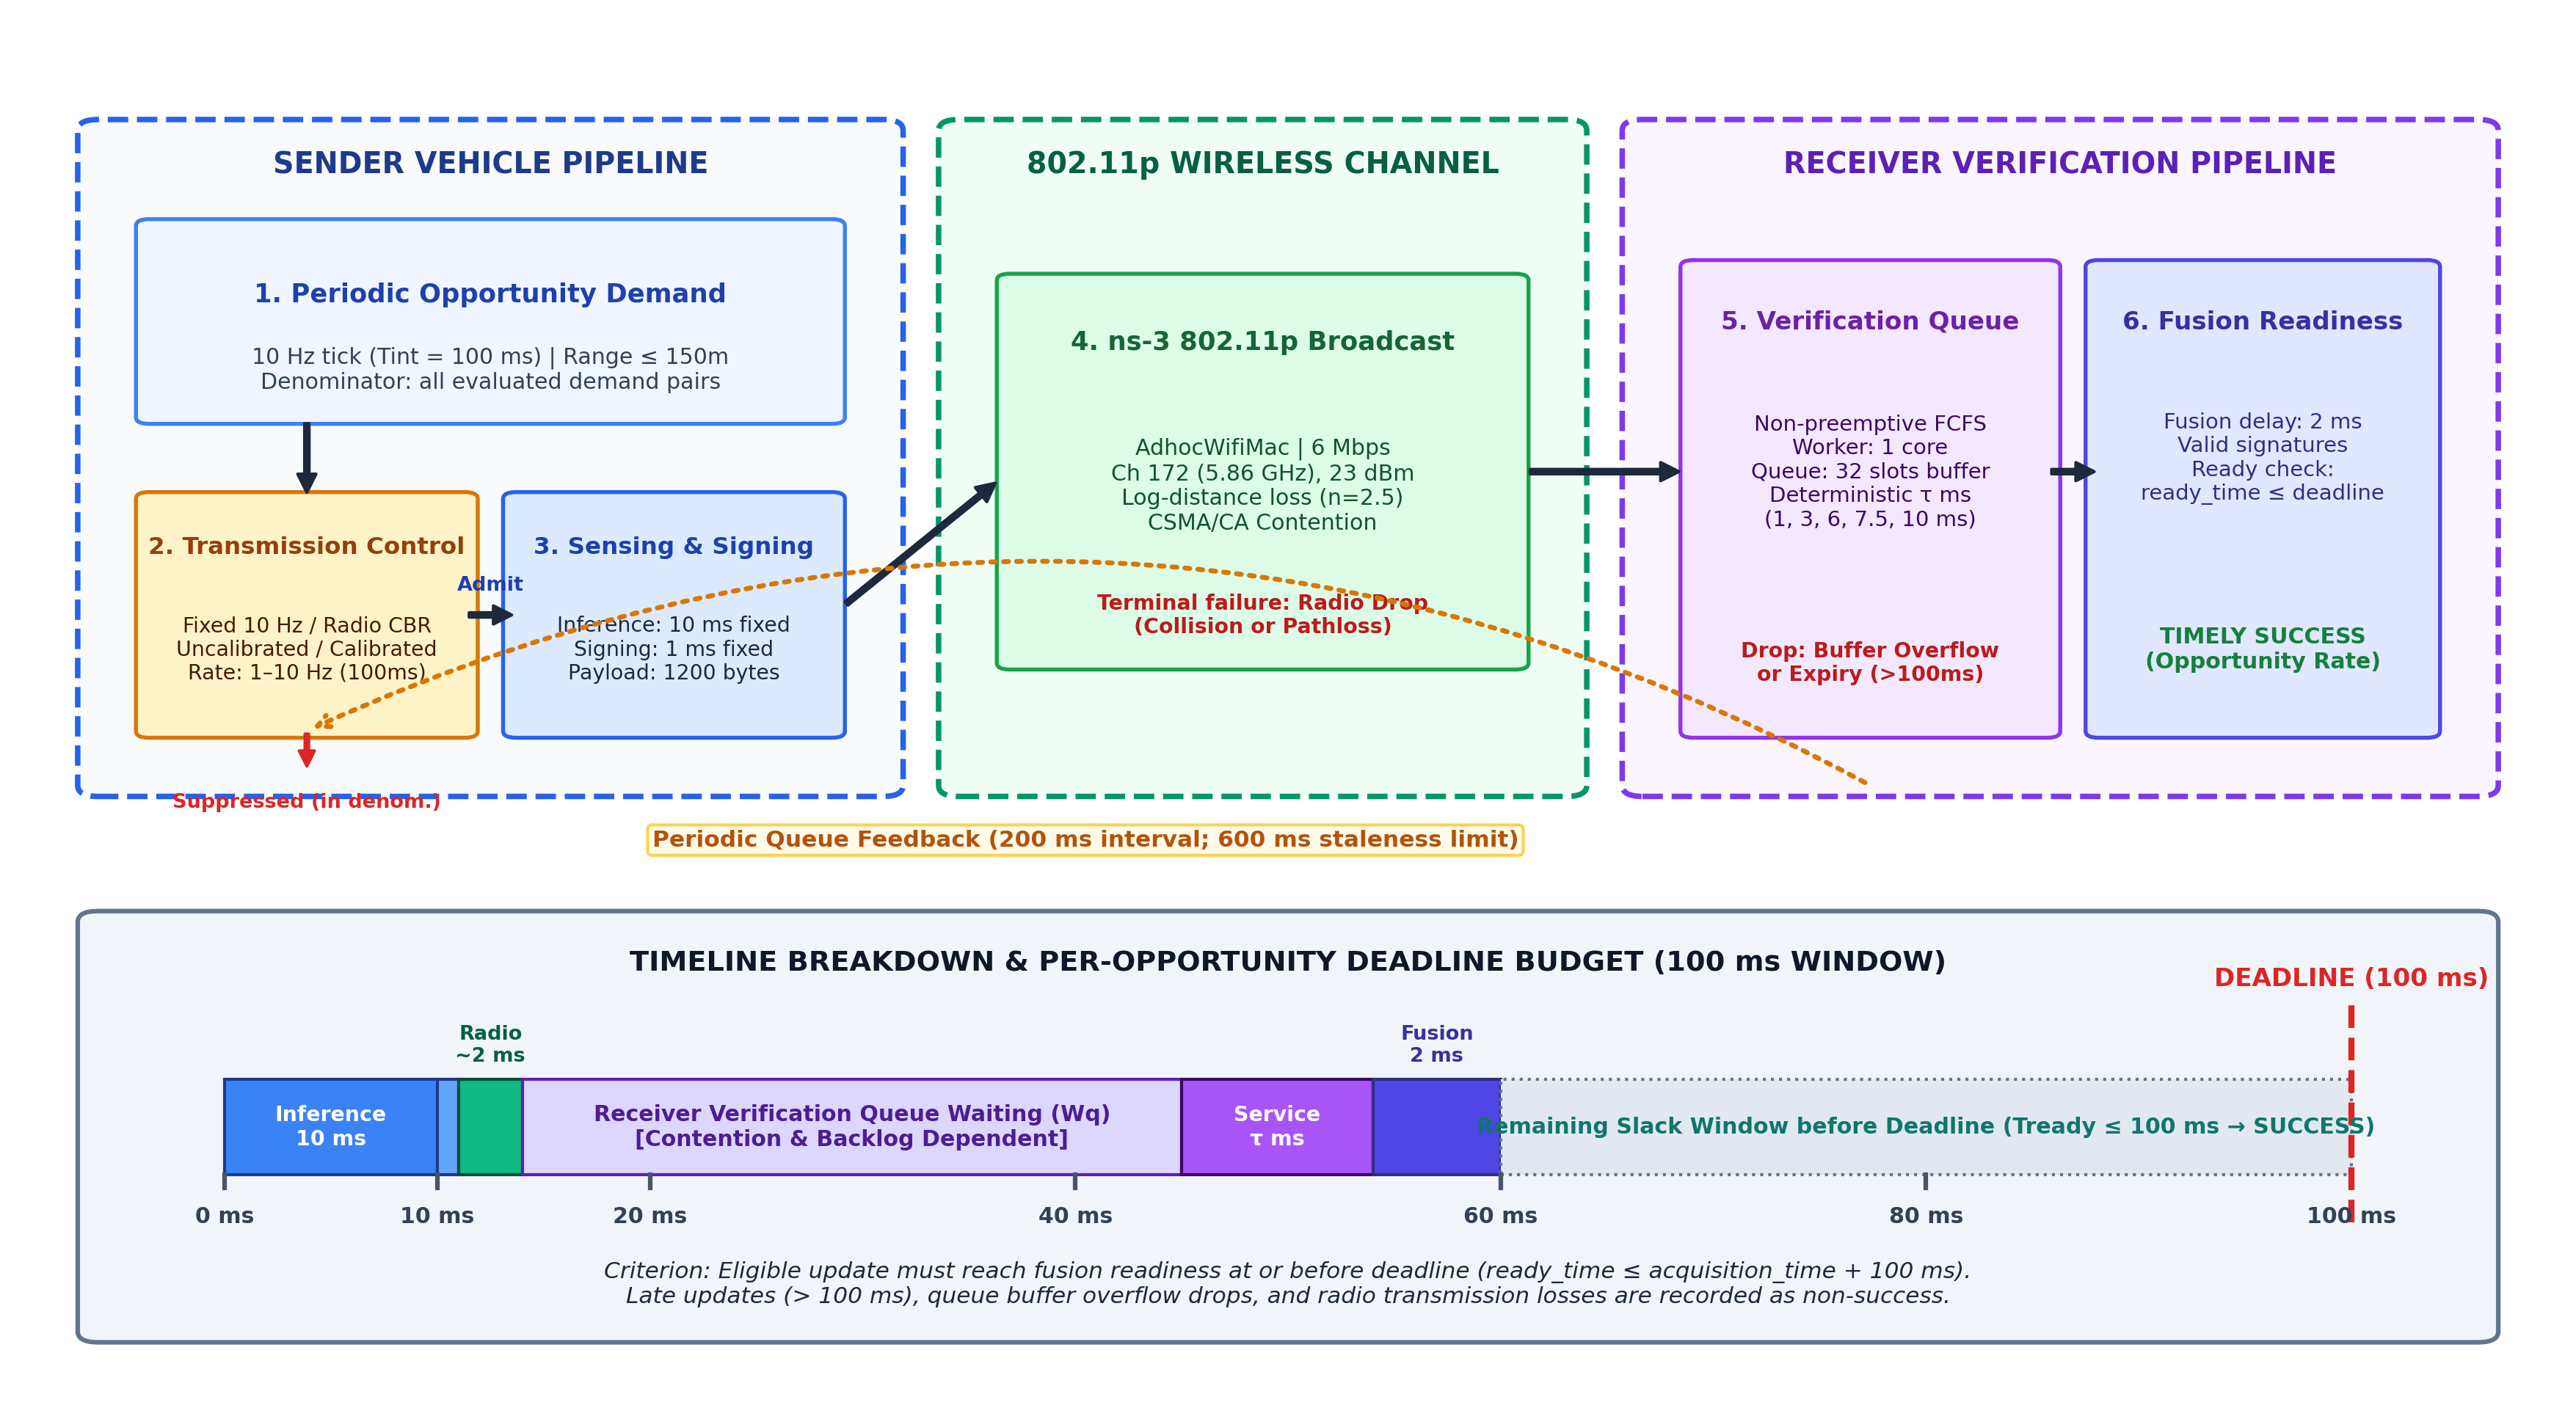
\includegraphics[keepaspectratio,alt={Figure 1: Simulated
cooperative-perception pipeline and verification timing
model.}]{figures/fig1_pipeline_timing.png}}
\caption{Figure 1: Simulated cooperative-perception pipeline and
verification timing model.}
\end{figure}

\textbf{Figure 1.} Simulated cooperative-perception pipeline and
verification timing model. Each periodic 10 Hz opportunity is either
admitted or suppressed; admitted updates traverse transmission, radio
propagation, receiver FCFS verification queue, and fusion delay before
the configured deadline.

The simulated deadline is 100 ms after acquisition and is a study
parameter, not a certified maneuver or safety deadline. For the primary
outcome, an eligible opportunity-receiver pair succeeds only when the
message generated for that exact opportunity reaches fusion readiness at
or before its deadline. Equality counts as success
(\texttt{ready\_time\ \textless{}=\ deadline}). The denominator is all
evaluated opportunity-receiver demand pairs, including suppressed
demand. Opportunities whose deadline falls beyond the observation stop
are excluded under the implementation's censoring rule.

We call this outcome the \textbf{same-opportunity timely success rate}
(the stored field \texttt{opportunity\_success\_rate}). It is not
object-level perception success, a safety measure, or an established
``TOSR'' metric. A separate \textbf{deadline freshness coverage} measure
(\texttt{opportunity\_freshness\_rate}) allows a later, fresher update
from the same source to satisfy an earlier opportunity's deadline query;
one update may cover multiple earlier queries. The two measures have
different credit rules and are not conflated in the results below. The
earlier draft's one-to-one opportunity-message matching proposition is
omitted because it does not describe the freshness-coverage rule.

For generated message-receiver pairs, terminal states include success,
radio not received, queue overflow, verification expiry, fusion expiry,
and unfinished/censored processing as applicable. This lifecycle
partition is distinct from the opportunity-receiver demand denominator,
because suppressed opportunities do not generate message-receiver pairs.
Independent replay validated conservation and saved-summary agreement
for 360 of 370 discovered runs. Ten stress runs have incomplete traces
and are not used for trace-supported stress aggregates.

\subsubsection{3.2. Receiver queue and offered
load}\label{receiver-queue-and-offered-load}

Each receiver has one non-preemptive FCFS verification worker and
capacity for 32 waiting messages, in addition to the active message.
Main-study service is deterministic (\texttt{service\_cv\ =\ 0}) and
configured between 1 and 10 ms depending on the experiment. Signatures
are assumed valid. The model does not implement ECDSA, certificate
parsing or validation, revocation, a VPKI, HSM/ECU scheduling, or
measured CPU execution. Frames are not pruned before verification;
expiry is checked after verification and after a fixed
fusion-availability delay. Fusion has no shared worker or GPU queue.

For the fixed-policy arrival analysis, receiver arrival rate \(\lambda\)
is counted from data receptions during \texttt{{[}1\ s,\ 5\ s)} and
divided by the 4 s interval. Offered load is calculated as
\(\rho=\lambda E[V]\), with the configured mean verification service
duration \(E[V]\). It is an offered-load estimate, not measured worker
busy fraction or a direct test of queue stability. The classical M/G/1
Pollaczek--Khinchine mean waiting-time formula
\(W_q=\lambda E[V^2]/(2(1-\rho))\) {[}11{]} assumes Poisson arrivals,
independent and identically distributed service times, FCFS discipline,
and an infinite waiting capacity with \(\rho<1\) (Kleinrock). The
simulation's periodic demand, radio contention, finite 32-slot queue,
and deterministic service do not establish those assumptions as a
predictive model for the empirical run traces. The expression is
conditional and analytical only.

\subsection{4. Policies and experiment
design}\label{policies-and-experiment-design}

All campaigns use common exogenous opportunity demand within each
prescribed comparison. The policies share configured rate bounds of
1--10 Hz and a 100 ms control interval where applicable. Rate admissions
are quantized to opportunity ticks, so controller targets need not equal
realized transmission rates exactly.

\begin{itemize}
\tightlist
\item
  \textbf{Fixed:} emits at the configured fixed rate (10 Hz in the
  primary comparison).
\item
  \textbf{Radio:} project-specific channel-busy-ratio AIMD rate
  controller. It is not identified as ETSI DCC.
\item
  \textbf{Receiver:} queue-feedback-only policy used in the factorial
  campaign.
\item
  \textbf{Joint:} combines radio occupancy and authenticated neighbor
  backlog reports; missing or stale feedback can trigger a conservative
  reduction under its coded rule.
\item
  \textbf{Calibrated:} a diagnostic feedback variant with modified
  thresholds and a cross-sectional arithmetic mean over currently fresh
  neighbor reports at each control update. It is not a temporal moving
  average and ``calibrated'' is the project's policy name, not hardware
  calibration.
\item
  \textbf{DCC:} project single-service mapping based on a bounded
  adaptive core and an airtime-to-interval rule. It is not a complete
  ETSI/ITS-G5 implementation and is excluded from the 20-seed paired
  study.
\end{itemize}

Four experiment families are kept distinct. The \textbf{factorial
campaign} contains 180 audited runs: two synthetic scenarios
(intersection/highway), 12/24/48 sources, 1/3 ms service, five policies
(fixed, radio, receiver, joint, DCC), and three seeds per cell
(101--103). The \textbf{verification stress sweep} was designed for 75
runs (48 sources, intersection, five service times: 1, 3, 6, 7.5, and 10
ms; five policies; three seeds). Sixty-five runs passed trace audit; ten
preserved traces are incomplete. The \textbf{threshold ablation} has 35
audited runs (seven conditions, five seeds); comparisons among
thresholds 4, 8, 16, and 24 are exploratory and outcome-informed. The
\textbf{paired comparison} has 80 audited runs: four policies (fixed,
radio, joint, calibrated), 20 paired seeds, 48 sources, intersection,
and 3 ms service. It contains no DCC policy. All campaigns are
exploratory; the paired design's replication does not establish
confirmatory status.

Historical major-revision records do not embed the exact source
revision, complete configuration hash, or simulator binary hash. The run
catalog and results reconciliation record this provenance limitation.
Raw records were preserved; corrected summaries are under
\texttt{results/processed/rework/}.

\subsection{5. Results}\label{results}

\subsubsection{5.1. Factorial campaign}\label{factorial-campaign}

All 180 factorial run records passed the terminal audit. Each condition
has three seed replications, so uncertainty is substantial and results
are descriptive. At the intersection setting with 48 sources and 3 ms
service, same-opportunity success was 95.28\% for fixed, 86.03\% for
radio, 13.30\% for joint, 13.30\% for receiver-only feedback, and
45.86\% for the project DCC mapping. The corresponding 95\% t interval
half-widths across three seeds were 1.79, 20.65, 1.71, 1.71, and 0.24
percentage points, respectively. This factorial cell is not the same
protocol or seed set as the separate paired study.

Across the full factorial, effects varied with source count, scenario,
service input, and policy. The three-seed design does not support broad
population estimates. The complete 60-cell table is available in
\texttt{results/processed/evaluation/results.csv} and
\texttt{summary.json}.

\emph{Provenance:} The 48-source intersection cell is the
3-run-per-policy subset of
\texttt{results/processed/evaluation/results.csv}; the denominator is
evaluated opportunity-receiver pairs as recorded in the corresponding
audited run summaries. The 95\% intervals are the saved across-seed
Student-t intervals.

\subsubsection{5.2. Offered receiver load}\label{offered-receiver-load}

The corrected fixed-policy arrival analysis includes all 48 receivers
over three seeds. In this analysis, offered load \(\rho = \lambda E[V]\)
is an analytical calculation applying several configured service
durations \(E[V]\) to a single common baseline of simulation-derived
packet-reception observations (\(\lambda = 190.422\)
packets/s/receiver), rather than from separate independent simulation
runs executed at each service duration. The two unavailable/truncated 3
ms traces were replaced with matching fixed-policy traces from the 1 ms
folder, whose observed receptions were identical where comparisons were
possible; this reuse is documented in the analysis output. Values
describe the sampled fixed-policy receptions, not a separately measured
processor utilization.

\textbf{Table 2. Fixed-policy receiver offered load (48 sources; 3
seeds; 144 receiver-seed observations)}

{\def\LTcaptype{none} % do not increment counter
\begin{longtable}[]{@{}
  >{\raggedleft\arraybackslash}p{(\linewidth - 10\tabcolsep) * \real{0.1667}}
  >{\raggedleft\arraybackslash}p{(\linewidth - 10\tabcolsep) * \real{0.1667}}
  >{\raggedleft\arraybackslash}p{(\linewidth - 10\tabcolsep) * \real{0.1667}}
  >{\raggedleft\arraybackslash}p{(\linewidth - 10\tabcolsep) * \real{0.1667}}
  >{\raggedleft\arraybackslash}p{(\linewidth - 10\tabcolsep) * \real{0.1667}}
  >{\raggedleft\arraybackslash}p{(\linewidth - 10\tabcolsep) * \real{0.1667}}@{}}
\toprule\noalign{}
\begin{minipage}[b]{\linewidth}\raggedleft
Service budget (ms)
\end{minipage} & \begin{minipage}[b]{\linewidth}\raggedleft
Mean arrivals (packets/s/receiver)
\end{minipage} & \begin{minipage}[b]{\linewidth}\raggedleft
Mean offered \(\rho\)
\end{minipage} & \begin{minipage}[b]{\linewidth}\raggedleft
Median \(\rho\)
\end{minipage} & \begin{minipage}[b]{\linewidth}\raggedleft
Maximum \(\rho\)
\end{minipage} & \begin{minipage}[b]{\linewidth}\raggedleft
Mean receivers per run with \(\rho>1\)
\end{minipage} \\
\midrule\noalign{}
\endhead
\bottomrule\noalign{}
\endlastfoot
1.0 & 190.422 & 0.190 & 0.218 & 0.304 & 0.00 \\
3.0 & 190.422 & 0.571 & 0.654 & 0.911 & 0.00 \\
6.0 & 190.422 & 1.143 & 1.309 & 1.823 & 29.67 \\
7.5 & 190.422 & 1.428 & 1.636 & 2.278 & 32.67 \\
10.0 & 190.422 & 1.904 & 2.181 & 3.038 & 38.00 \\
\end{longtable}
}

The calculation places mean offered load below one at 3 ms and above one
at 6 ms under these fixed-policy traces. It does not by itself establish
a physical bottleneck transition, worker saturation, deadline failure,
or causality. At 3 ms no receiver-seed observation exceeded one in the
recomputed sample; the earlier manuscript values were inflated by an
observation-window mismatch.

\begin{figure}
\centering
\pandocbounded{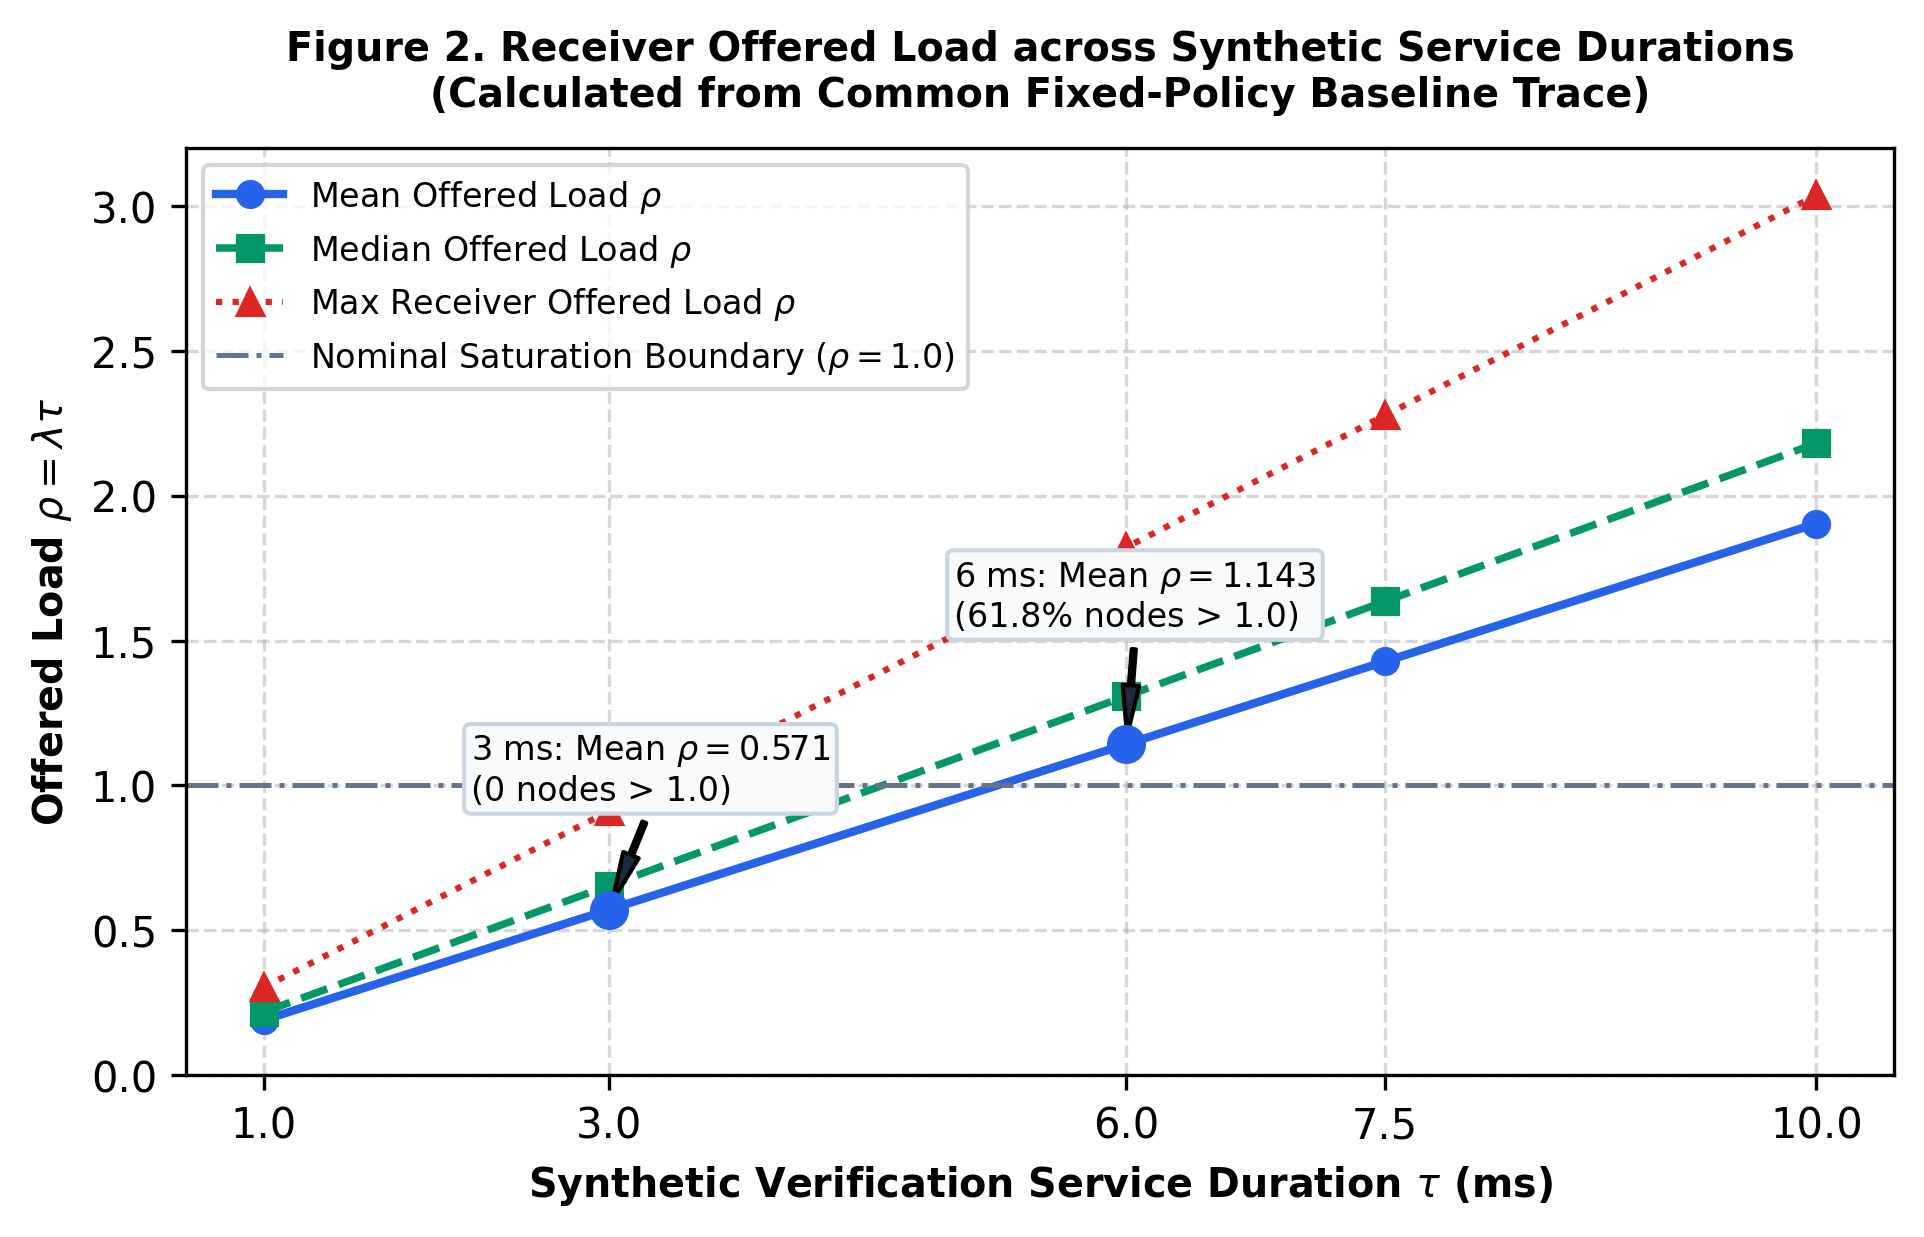
\includegraphics[keepaspectratio,alt={Figure 2: Receiver
offered load across synthetic verification service
budgets.}]{figures/fig2_offered_load.png}}
\caption{Figure 2: Receiver offered load across synthetic verification
service budgets.}
\end{figure}

\textbf{Figure 2.} Receiver offered load \(\rho = \lambda E[V]\)
calculated across synthetic verification service budgets from a common
fixed-policy reception-rate baseline (144 receiver observations across 3
seeds). Offered load is an analytical calculation applying configured
service durations to the same observed arrival rates, not independent
runs or measured CPU execution. Dashed red line denotes the theoretical
saturation threshold (\(\rho = 1.0\)).

\emph{Provenance:} \texttt{scripts/recompute\_utilization.py},
\texttt{results/processed/rework/utilization\_recomputed.json}, and
\texttt{utilization\_by\_receiver.csv}; each budget evaluates 48
receivers × 3 seeds (144 receiver-seed observations) by applying service
duration \(\tau\) to the common fixed-policy reception baseline. The 3
ms input includes two explicitly disclosed baseline-trace reuses.

\subsubsection{5.3. Stress sweep}\label{stress-sweep}

Stress estimates use only trace-audited runs and report the
cell-specific number of runs. The 3 ms calibrated cell has two audited
seeds; the 6 ms calibrated cell has one. Cells with one run have no
estimable across-seed confidence interval. These exploratory
observations must not be read as complete three-seed comparisons.

\textbf{Table 3. Selected trace-audited stress outcomes}

{\def\LTcaptype{none} % do not increment counter
\begin{longtable}[]{@{}
  >{\raggedleft\arraybackslash}p{(\linewidth - 8\tabcolsep) * \real{0.2105}}
  >{\raggedright\arraybackslash}p{(\linewidth - 8\tabcolsep) * \real{0.1579}}
  >{\raggedleft\arraybackslash}p{(\linewidth - 8\tabcolsep) * \real{0.2105}}
  >{\raggedleft\arraybackslash}p{(\linewidth - 8\tabcolsep) * \real{0.2105}}
  >{\raggedleft\arraybackslash}p{(\linewidth - 8\tabcolsep) * \real{0.2105}}@{}}
\toprule\noalign{}
\begin{minipage}[b]{\linewidth}\raggedleft
Service (ms)
\end{minipage} & \begin{minipage}[b]{\linewidth}\raggedright
Policy
\end{minipage} & \begin{minipage}[b]{\linewidth}\raggedleft
Audited n
\end{minipage} & \begin{minipage}[b]{\linewidth}\raggedleft
Same-opportunity success (\%)
\end{minipage} & \begin{minipage}[b]{\linewidth}\raggedleft
95\% t interval half-width (pp)
\end{minipage} \\
\midrule\noalign{}
\endhead
\bottomrule\noalign{}
\endlastfoot
3 & Calibrated & 2 & 53.04 & 13.49 \\
3 & Joint & 3 & 11.42 & 6.05 \\
3 & Radio & 3 & 77.32 & 13.28 \\
3 & DCC mapping & 3 & 43.80 & 4.93 \\
6 & Calibrated & 1 & 3.54 & Not estimable \\
6 & Joint & 2 & 2.74 & 13.60 \\
6 & DCC mapping & 3 & 43.26 & 4.53 \\
\end{longtable}
}

The stress sweep shows that observed outcomes differ across tested
policies and configured service budgets. Incomplete traces, small cell
sizes, and the synthetic deterministic service model preclude a broad
mechanism claim. The full recomputed cell data, including all verified n
values, are in \texttt{stress\_recomputed.csv}.

\emph{Provenance:} \texttt{scripts/reconcile\_results.py} and
\texttt{results/processed/rework/stress\_recomputed.csv}; rates use each
run's evaluated opportunity-receiver denominator and only
terminal-audited runs. The \texttt{n} column is the audited
independent-run count for each policy/service cell.

\subsubsection{5.4. Threshold ablation}\label{threshold-ablation}

All 35 ablation runs passed the trace audit. This was an exploratory
comparison at 48 sources, intersection geometry, and 3 ms service. The
threshold outcomes were examined in the same study and do not
independently validate a selected threshold.

\textbf{Table 4. Five-seed threshold ablation}

{\def\LTcaptype{none} % do not increment counter
\begin{longtable}[]{@{}
  >{\raggedright\arraybackslash}p{(\linewidth - 6\tabcolsep) * \real{0.2000}}
  >{\raggedleft\arraybackslash}p{(\linewidth - 6\tabcolsep) * \real{0.2667}}
  >{\raggedleft\arraybackslash}p{(\linewidth - 6\tabcolsep) * \real{0.2667}}
  >{\raggedleft\arraybackslash}p{(\linewidth - 6\tabcolsep) * \real{0.2667}}@{}}
\toprule\noalign{}
\begin{minipage}[b]{\linewidth}\raggedright
Condition
\end{minipage} & \begin{minipage}[b]{\linewidth}\raggedleft
n
\end{minipage} & \begin{minipage}[b]{\linewidth}\raggedleft
Mean same-opportunity success (\%)
\end{minipage} & \begin{minipage}[b]{\linewidth}\raggedleft
95\% t interval half-width (pp)
\end{minipage} \\
\midrule\noalign{}
\endhead
\bottomrule\noalign{}
\endlastfoot
Fixed 10 Hz & 5 & 94.06 & 2.83 \\
Radio-only & 5 & 81.49 & 9.88 \\
Uncalibrated joint & 5 & 13.01 & 3.73 \\
Queue threshold 4 & 5 & 21.37 & 9.33 \\
Queue threshold 8 & 5 & 47.42 & 12.78 \\
Queue threshold 16 & 5 & 55.31 & 3.80 \\
Queue threshold 24 & 5 & 54.29 & 4.62 \\
\end{longtable}
}

Threshold 16 had the largest observed mean among the four tested
thresholds in this five-seed ablation. This is a descriptive,
outcome-informed result, not evidence that 16 is optimal outside the
tested candidates or setting.

\emph{Provenance:}
\texttt{results/processed/rework/ablation\_recomputed.csv}; each listed
condition has five audited runs, and the mean and 95\% t interval are
computed over run-level same-opportunity rates.

\subsubsection{5.5. Paired comparison}\label{paired-comparison}

All 80 records passed terminal conservation and summary reconciliation.
This comparison uses the same 20 seeds for four policies at 48 sources,
intersection geometry, and 3 ms service. Values below are means over
seed-level same-opportunity success; intervals are 95\% Student-t
intervals over those seed-level values. Policy means and paired
contrasts are both reported so the paired design is explicit.

\textbf{Table 5. Twenty-seed paired policy comparison}

{\def\LTcaptype{none} % do not increment counter
\begin{longtable}[]{@{}lrrr@{}}
\toprule\noalign{}
Policy & n & Mean success (\%) & 95\% CI half-width (pp) \\
\midrule\noalign{}
\endhead
\bottomrule\noalign{}
\endlastfoot
Fixed 10 Hz & 20 & 94.75 & 0.98 \\
Radio & 20 & 81.98 & 3.95 \\
Joint & 20 & 15.84 & 6.54 \\
Calibrated feedback & 20 & 55.91 & 4.37 \\
\end{longtable}
}

\textbf{Table 6. Paired differences in same-opportunity success}

{\def\LTcaptype{none} % do not increment counter
\begin{longtable}[]{@{}
  >{\raggedright\arraybackslash}p{(\linewidth - 6\tabcolsep) * \real{0.2000}}
  >{\raggedleft\arraybackslash}p{(\linewidth - 6\tabcolsep) * \real{0.2667}}
  >{\raggedleft\arraybackslash}p{(\linewidth - 6\tabcolsep) * \real{0.2667}}
  >{\raggedleft\arraybackslash}p{(\linewidth - 6\tabcolsep) * \real{0.2667}}@{}}
\toprule\noalign{}
\begin{minipage}[b]{\linewidth}\raggedright
Contrast
\end{minipage} & \begin{minipage}[b]{\linewidth}\raggedleft
Mean paired difference (pp)
\end{minipage} & \begin{minipage}[b]{\linewidth}\raggedleft
95\% paired t interval half-width (pp)
\end{minipage} & \begin{minipage}[b]{\linewidth}\raggedleft
Cohen's \(d_z\)
\end{minipage} \\
\midrule\noalign{}
\endhead
\bottomrule\noalign{}
\endlastfoot
Calibrated − joint & +40.07 & 4.18 & 4.49 \\
Calibrated − fixed & −38.83 & 4.49 & −4.05 \\
Calibrated − radio & −26.07 & 2.74 & −4.45 \\
\end{longtable}
}

At this operating point, calibrated feedback had higher mean
same-opportunity success than uncalibrated joint feedback and lower mean
success than fixed and radio policies. These are contrasts among the
implemented policies in one synthetic configuration. They do not
establish universal controller ranking or real-world perception effects.
The project's radio policy is not ETSI DCC.

\begin{figure}
\centering
\pandocbounded{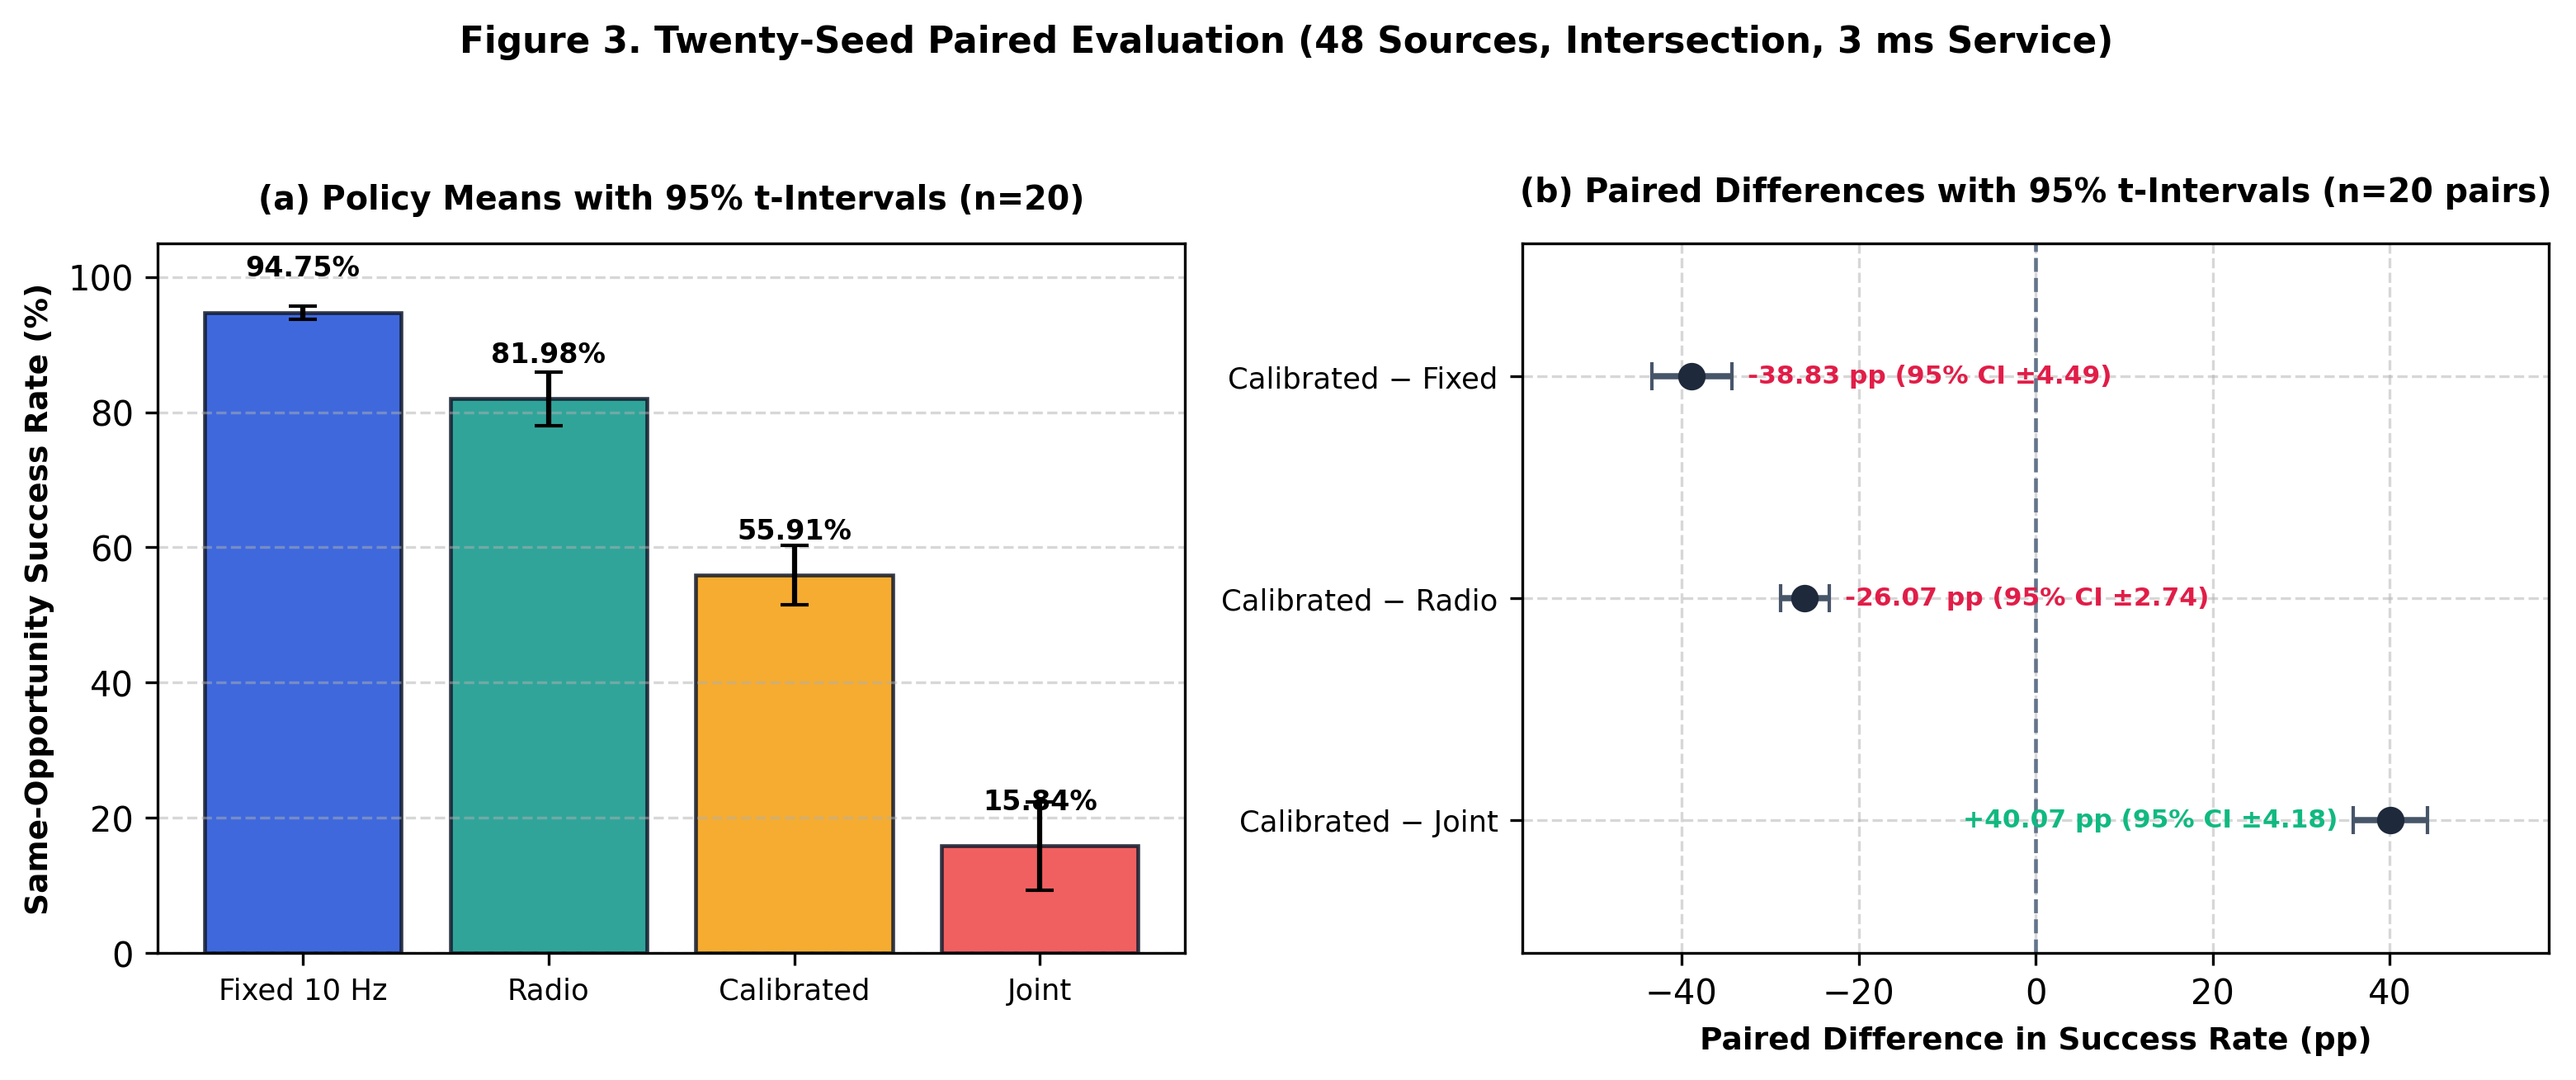
\includegraphics[keepaspectratio,alt={Figure 3:
Twenty-seed paired policy
evaluation.}]{figures/fig3_paired_comparison.png}}
\caption{Figure 3: Twenty-seed paired policy evaluation.}
\end{figure}

\textbf{Figure 3.} Twenty-seed paired policy evaluation (48 sources,
intersection scenario, 3 ms service). (a) Mean same-opportunity timely
success rate with 95\% Student-t confidence intervals across policies.
(b) Mean paired differences with 95\% paired Student-t confidence
intervals relative to uncalibrated joint feedback, fixed 10 Hz, and
radio-only control.

\emph{Provenance:} Policy means and intervals:
\texttt{results/processed/rework/paired\_policy\_recomputed.csv}; paired
differences, intervals, and Cohen's dz:
\texttt{results/processed/rework/paired\_contrasts\_recomputed.csv}.
Each policy uses 20 audited runs; each contrast uses 20 matched seed
pairs. The per-run rate denominator is evaluated opportunity-receiver
pairs.

\subsubsection{5.6. Trigger attribution}\label{trigger-attribution}

In the saved trigger-attribution record, 1,242 of 1,330 observed rate
decreases for the uncalibrated joint policy (93.38\%) were classified as
\texttt{backlog\_only}. This is a descriptive classification of
controller decisions. It does not establish that reports were isolated
outliers or that this trigger category caused the aggregate performance
difference. The attribution source and decision denominator are recorded
in \texttt{evidence/claim\_evidence.csv}.

\emph{Provenance:}
\texttt{results/raw/major\_revision/trigger\_attribution.json};
denominator is 1,330 observed rate-decrease decisions, not messages or
opportunities.

\subsection{6. Discussion}\label{discussion}

The paired experiment shows that delayed receiver-load feedback changed
the measured same-opportunity outcome in the tested simulation:
calibrated feedback had greater success than the uncalibrated joint
policy, but less than fixed transmission and the project radio policy.
The factorial and ablation results show substantial policy and setting
variation, while the stress sweep has incomplete cells. Taken together,
they motivate further controlled study of feedback policy behavior; they
do not support a general recommendation for or against receiver
feedback.

One conditional service-load calculation can illustrate why offered
demand and service time matter. If one receiver has exactly 24 equally
active senders, every update is received without loss, each update
consumes deterministic service \(\tau\), and service is equally
allocated, offered load below one requires each sender rate
\(f < 1/(24\tau)\). For \(\tau=6\) ms, this is \(f<6.94\) Hz. This
arithmetic is not a bound on same-opportunity success, not a theorem
about the simulated system, and not a prediction: the simulation has
dynamic neighborhoods, radio losses, nonuniform arrival rates, feedback
traffic, and finite queues.

A next study that could change the interpretation would independently
vary feedback delay, loss, report staleness, worker count, queue
capacity, service-time variability, payload and radio conditions, while
preserving paired common demand and complete run provenance. It should
also measure hardware service distributions if the intended inference
concerns cryptographic implementations. Object-level perception and
safety questions require separate validated perception and hazard
outcomes.

\subsection{7. Model settings and
limitations}\label{model-settings-and-limitations}

\textbf{Table 7. Implemented model settings and interpretation limits}

{\def\LTcaptype{none} % do not increment counter
\begin{longtable}[]{@{}
  >{\raggedright\arraybackslash}p{(\linewidth - 4\tabcolsep) * \real{0.3333}}
  >{\raggedright\arraybackslash}p{(\linewidth - 4\tabcolsep) * \real{0.3333}}
  >{\raggedright\arraybackslash}p{(\linewidth - 4\tabcolsep) * \real{0.3333}}@{}}
\toprule\noalign{}
\begin{minipage}[b]{\linewidth}\raggedright
Component
\end{minipage} & \begin{minipage}[b]{\linewidth}\raggedright
Implemented setting
\end{minipage} & \begin{minipage}[b]{\linewidth}\raggedright
Interpretation limit
\end{minipage} \\
\midrule\noalign{}
\endhead
\bottomrule\noalign{}
\endlastfoot
Simulator/radio & ns-3.46.1; 802.11p PHY with AdhocWifiMac {[}9, 10{]};
6 Mbps, 10 MHz, channel 172, 23 dBm & Configured simulation only; no
full ITS-G5 stack or field calibration \\
Propagation & Log-distance loss, exponent 2.5, reference loss 47.86 dB;
constant-speed propagation delay {[}10{]} & No building blockage,
shadowing, calibrated NLOS, or measured channel traces \\
Mobility/scenarios & Synthetic intersection and six-lane highway flows;
constant 10 m/s in both; node recycling & No SUMO, car following,
traffic lights, or measured trajectories \\
Demand/eligibility & Periodic 10 Hz opportunities; 100 ms configured
deadline; 150 m eligibility geometry & No object detections; deadline is
not a certified safety deadline; eligibility differs from radio
reception \\
Data and feedback & 1100-byte synthetic data payload plus 100-byte
modeled security overhead; 96-byte feedback payload plus modeled
overhead; feedback every 200 ms; 600 ms staleness limit & Not encoded
CPM or measured signed-message sizes; feedback shares radio and
verification resources \\
Processing & Fixed 10 ms inference, 1 ms signing, configured
deterministic verification (1--10 ms), fixed 2 ms fusion availability &
Synthetic delays; no sensor execution, signing/verification
implementation, certificate processing, or shared fusion/GPU worker \\
Receiver & One non-preemptive FCFS verification worker; 32 waiting slots
plus active message; signatures assumed valid & No measured CPU
utilization; no pre-verification expiry pruning; cannot generalize queue
rule to vehicle firmware \\
Control & 100 ms updates; project radio thresholds 0.65/0.40, rate
decrease multiplier 0.8, increase 0.5 Hz; queue thresholds vary by
policy/experiment & Project controller settings, not standard-mandated
values; timing is quantized to opportunity ticks \\
Evidence & 180 factorial, 65 trace-audited stress, 35 ablation, 80
paired runs & All analyses exploratory; historical stress/ablation
source, config, and binary hashes are incomplete \\
\end{longtable}
}

The principal limits are: (1) synthetic deterministic service times with
no cryptographic execution or hardware benchmark; (2) valid signatures
assumed, with no certificate-chain, revocation, or VPKI behavior; (3)
one receiver worker and no shared fusion/GPU queue; (4) no
pre-verification pruning and no measured processor busy time; (5)
synthetic payloads and fixed inference, signing, and fusion delays; (6)
constant-speed synthetic geometry rather than measured traffic; (7)
simplified propagation without blockage, shadowing, or measured
channels; (8) periodic demand rather than a Poisson process; (9) a
configured 100 ms timing threshold without safety interpretation; (10)
no perception accuracy, object tracking, collision, or safety endpoint;
(11) finite scenarios, selected seeds, and small replication in
factorial/stress/ablation cells; (12) incomplete raw traces for ten
stress runs; (13) offered-load estimates are not worker utilization;
(14) project \texttt{radio} and \texttt{dcc} labels are not
interchangeable, and \texttt{dcc} is not a conformance implementation;
(15) no broad sensitivity sweep across service variability, worker
count, queue capacity, radio range, payload, or feedback failures; and
(16) incomplete embedded source/configuration/binary provenance for
historical major-revision runs. These boundaries define the scope of
every result in this paper.

\subsection{8. Conclusion}\label{conclusion}

In this controlled simulation, fixed transmission and the project radio
controller had higher same-opportunity success than both feedback
policies in the 20-seed paired comparison at 48 sources, intersection
geometry, and 3 ms synthetic verification service. Calibrated feedback
improved the outcome relative to uncalibrated joint feedback, but did
not reach the fixed or radio means. The paired contrast is exploratory
and applies to this implementation and setting. Separate experiments
show varying outcomes across tested configurations; incomplete stress
traces and small cell sizes limit interpretation. The receiver
offered-load calculation gives mean \(\rho=0.571\) at 3 ms and \(1.143\)
at 6 ms under the analyzed fixed-policy traces, not measured CPU
utilization. Additional sensitivity experiments, complete provenance,
and hardware or perception measurements would be needed to assess
whether these patterns persist under other conditions. No conclusion
about vehicle safety, deployment performance, hardware verification
costs, or standards changes follows from the present study.

\subsection{CRediT authorship contribution
statement}\label{credit-authorship-contribution-statement}

\textbf{Dipesh Gurung:} Conceptualization, Methodology, Software, Formal
Analysis, Investigation, Data Curation, Writing -- original draft,
Visualization, Project administration.\\
\textbf{Binod Bhattarai:} Conceptualization, Investigation, Validation,
Writing -- review \& editing, Supervision.\\
\textbf{Prof.~Dr.~R. N. Thakur:} Conceptualization, Supervision,
Methodology, Resources, Writing -- review \& editing.

\subsection{Declaration of competing
interest}\label{declaration-of-competing-interest}

The authors declare that they have no known competing financial
interests or personal relationships that could have appeared to
influence the work reported in this paper.

\subsection{Declaration of generative AI in scientific
writing}\label{declaration-of-generative-ai-in-scientific-writing}

During the preparation of this work the authors used Google DeepMind's
Antigravity AI assistant in order to assist with manuscript formatting,
LaTeX conversion, syntax checking, and reproducible verification
scripting. After using this tool/service, the authors reviewed and
edited the content as needed and take full responsibility for the
content of the publication.

\subsection{Acknowledgements}\label{acknowledgements}

The authors thank the Department of Research and the Intel AI Unnati Lab
at Lord Buddha Education Foundation (LBEF College), Kathmandu, Nepal,
for providing computational infrastructure, research facilities, and lab
resources. The authors also thank the School of Sciences at Noida
International University for institutional support.

\subsection{Funding}\label{funding}

This research did not receive any specific grant from funding agencies
in the public, commercial, or not-for-profit sectors.

\subsection{Data availability}\label{data-availability}

Simulation code, configuration files, processed evaluation datasets, and
reproducible audit scripts are archived and publicly available at GitHub
repository: https://github.com/Dips7/cpstudy.

\subsection{References}\label{references}

\begin{enumerate}
\def\labelenumi{\arabic{enumi}.}
\tightlist
\item
  Thandavarayan, G., Sepulcre, M., \& Gozalvez, J. (2020). ``Cooperative
  Perception for Connected and Automated Vehicles: Evaluation and Impact
  of Congestion Control.'' \emph{IEEE Access}, 8, 197665--197683.
  https://doi.org/10.1109/ACCESS.2020.3035119.
\item
  Thandavarayan, G., Sepulcre, M., \& Gozalvez, J. (2020). ``Generation
  of Cooperative Perception Messages for Connected and Automated
  Vehicles.'' \emph{IEEE Transactions on Vehicular Technology}, 69(12),
  16336--16341. https://doi.org/10.1109/TVT.2020.3036165.
\item
  ETSI. (2023). \emph{Intelligent Transport System (ITS); Vehicular
  Communications; Basic Set of Applications; Collective Perception
  Service; Release 2}. ETSI TS 103 324 V2.1.1.
\item
  ETSI. (2018). \emph{Intelligent Transport Systems (ITS); Decentralized
  Congestion Control Mechanisms for Intelligent Transport Systems
  operating in the 5 GHz range; Access layer part}. ETSI TS 102 687
  V1.2.1.
\item
  Muhammad, M., Kearney, P., Aneiba, A., \& Kunz, A. (2019). ``Analysis
  of Security Overhead in Broadcast V2V Communications.'' In
  \emph{Computer Safety, Reliability, and Security Workshops (SAFECOMP
  2019 Workshops)}, LNCS 11693, 251--263.
  https://doi.org/10.1007/978-3-030-26250-1\_20.
\item
  Wang, L., Sun, J., Sun, Y., Zhou, S., \& Niu, Z. (2023). ``Age of
  Information Guaranteed Scheduling for Asynchronous Status Updates in
  Collaborative Perception.'' In \emph{Proceedings of the 21st
  International Symposium on Modeling and Optimization in Mobile, Ad
  Hoc, and Wireless Networks (WiOpt 2023)}, 1--8.
  https://doi.org/10.23919/WiOpt58741.2023.10349877. Also available as
  arXiv:2310.04813.
\item
  Chen, X., Zhuang, Y., \& Yang, K. (2025). ``Age of Computing: A Metric
  of Computation Freshness in Communication and Computation Cooperative
  Networks.'' \emph{IEEE Transactions on Mobile Computing}, 24(11),
  11987--12000. https://doi.org/10.1109/TMC.2025.3582741. Also available
  as arXiv:2403.05007.
\item
  Tian, J., Shi, Y., \& Chen, S. (2026). ``Sense2Com: Coordinating
  sensing, communication, and computation for V2V cooperative
  perception.'' \emph{Physical Communication}, 78, 103214.
  https://doi.org/10.1016/j.phycom.2026.103214.
\item
  Henderson, T. R., Lacage, M., Riley, G. F., Dowell, C., \& Kopena, J.
  (2008). ``Network simulations with the ns-3 simulator.'' In
  \emph{Proceedings of the ACM SIGCOMM 2008 Conference (SIGCOMM '08)},
  527. https://doi.org/10.1145/1402958.1403014.
\item
  ns-3 project. (2025). \emph{ns-3.46.1 Release Information and ns-3.46
  Model Library Documentation}. ns-3 Consortium. Release:
  https://www2.nsnam.org/releases/ns-3-46/download/; Model
  documentation:
  https://www.nsnam.org/docs/release/3.46/models/html/wifi-user.html.
\item
  Kleinrock, L. (1975). \emph{Queueing Systems, Volume I: Theory}. John
  Wiley \& Sons, New York.
\end{enumerate}

\end{document}
